% Chapter 3
\chapter{Modeling single-neuron activations via nonparametric mixtures}
\chaptermark{Modeling single-neuron activations via nonparametric mixtures}

\vspace{.7cm}
As discussed in Section~\ref{ch1_sec:spike_train_analysis}, routine methods to analyze calcium imaging data are based on a two-step approach. 
However, it is expected the rate and the distribution of spikes to be stimulus-dependent \citep{Brenner2002PhysRevE}, but none of the previously described approaches allows to take into account explicitly the heterogeneity of spikes' behaviors as a function of the stimulus. 
As Figure~\ref{ch1_fig:trace_neurons} clearly shows for the Allen Brain Observatory data, the spikes' intensities vary greatly according to the type of stimulus.

In this chapter, we introduce a coherent nested Bayesian finite mixture model that allows for the estimation of the spiking activity of each neuron -- which could be seen as a first step for the analysis of larger brain activity combining multiple neurons in a region. In addition, our model \textit{simultaneously} allows for reconstructing the distributions of spikes under various experimental conditions; for example, in response to different types of visual stimuli in the Allen Brain Observatory data set. 

More specifically, our modeling framework estimates and clusters the distributions of the calcium transient spikes' amplitudes via a nested formulation of the generalized mixture of finite mixtures (gMFM) prior recently proposed by \citet{fruhwirthschnatter2020}. 
The proposed model further adopts the use of a common atom specification as in \citet{denti2021} for estimating the distribution of the spikes' amplitudes under each experimental condition. The proposed common atom gMFM has several advantages with respect to typical Bayesian nonparametric models for nested data. With respect to models based on Dirichlet process priors, the gMFM provides increased flexibility to estimate partitions characterized either by many, well-balanced, clusters or by a small set of large clusters. The common atom model allows to obtain nested inference on densities without incurring in the degeneracy issues pointed out by \citet{camerlenghi2019} for the widely used nested Dirichlet process of \citet{rodriguez2008}. At the same time, the common atom formulation still leverages two nested layers of random discrete mixture priors to borrow information between experiments and to identify similarities in the distributional patterns of the neuronal responses to different stimuli. In addition, differently than in the nested Dirichlet process, the common atom model also allows to cluster the inferred spikes' intensity values both within and between experimental conditions, so to infer common (recurring) response amplitudes. Finally, we allow our model to enforce sparsity of neuron firing over time by assuming a spike-and-slab prior specification on the marginal distribution of the amplitudes.


%\section{Mixture model for nested calcium imaging data}
\section{Model and prior specification}
\label{s:model}

We consider the biophysical model for the calcium dynamics~\eqref{ch1_eq:armodel} introduced in Section~\ref{ch1_sec:deconvolution_methods}, and the interpretation of the $A_t$ parameters as \textit{amplitude} of a spike at time $t$, taking value $0$ if there is no spike and a positive value otherwise.

We are interested in characterizing the neuronal activity under different experimental conditions. For each time point $t=1,\dots,T$, let $g_t$ be a discrete categorical variable, taking values in $\{1,\dots, J\}$, where $J$ is the number of distinct experimental settings, so that $g_t=j$ indicates that the neuronal activity at time $t$ is observed under condition $j$. The experimental conditions are often designed to capture variations in neuronal activity with respect to a baseline process, which may represent a ``typical" brain process. For example, in the Allen Observatory data, the interest is to investigate visually-evoked functional responses of neurons in the mouse's visual cortex. Therefore, neurons associated with visual decoding should be expected to activate in all conditions. It is then of interest to study not only \textit{if} but also \textit{how} the neurons differentially respond to the presentation of a variety of visual stimuli. 

In this chapter, we propose a hierarchical Bayesian approach to investigate similarities and differences in the distribution of spikes over time and conditions. In order to borrow information across different experimental conditions, one option is to fit a parametric hierarchical random effect model, and obtain a post-MCMC clustering of the estimated spikes $A_t$ by grouping together those spikes with similar magnitudes. This approach has several limitations: on the one hand, the distribution of the random effects is constrained into a specific parametric form; on the other hand, the clustering of, say, the posterior mean estimates of the parameters $A_t$'s does not allow to fully describe stimulus-specific distributional differences and to take into account the posterior uncertainty in the spikes.

In order to allow flexible modeling of distributions and to describe the heterogeneity of distributional features, we assume a nested Bayesian finite mixture specification. More specifically, we rewrite~\eqref{ch1_eq:armodel} as
\begin{equation*}
y_t\mid b, \gamma, \Ca_{t-1}, A_t, \sigma^2, \tau^2 \sim \N(b+\gamma\:\Ca_{t-1} + A_t, \sigma^2 + \tau^2 )
\end{equation*}
and we assume that the spikes $A_t$ are from stimulus-specific distributions, i.e. 
$ (A_t \mid g_t = j, \, G_j) \sim G_j$, $ j=1, \ldots, J$,
to account for the observed variety of neuronal activity under different experiment settings. We further allow for clustering the distributions across conditions, in order to capture similar patterns of neuronal activity. Indeed, one may typically expect $K<J$ distributional clusters. For example, a neuron may respond to general visual stimulation and not specifically to the type of stimulus considered. More specifically, we assume the following generalized mixture of finite mixtures structure:
%
\begin{equation}
G_1,\dots,\,G_J \mid Q \sim Q, \qquad Q = \sum_{k=1}^{K} \pi_k \delta_{G^*_k}
\label{eq:first_layer}
\end{equation}
where \(\pi_1,\dots,\pi_K \mid K \sim \Dir_K\left(\alpha/K, \ldots \alpha/K\right)\), $\alpha>0$, and $G_1^*, \ldots, G_K^*$ are a set of cluster-defining distributions, obtained as realizations of an underlying random probability measure, specified further below. Equation \eqref{eq:first_layer} implies that the $G_j$'s, $j=1,\ldots, J$ have a positive probability of clustering together, thereby giving rise to \textit{distributional clusters}. In practice, the number of mixture components, $K$, is typically larger than the number of clusters, $K_+$, and some of the atoms $G_k^*$ are not assigned to any of the $G_j$'s (empty components). The prior on the number of mixture components $K$ is a translated beta-negative-binomial distribution as in \citet{fruhwirthschnatter2020}. 
Including a prior $p(K)$ leads to both $K_+$ and $K$ being random a priori. 
Finally, the distributional atoms $G_k^*$, $k=1, \ldots, K$ are also obtained as a realization from an underlying generalized mixture of finite mixtures, 
\begin{equation}
G^*_k = \sum_{l=1}^{L} \omega_{l,k} \delta_{A^*_l}
\label{eq:second_layer}
\end{equation}
with $\omega_{1,k},\dots,\omega_{L,k} \mid L\sim \Dir_L\left(\beta/L\right)$, for some positive real number $\beta>0$. The set of atoms $A_l^*$ is common across all distributions $G_1^*, \ldots, G_K^*$ and they are obtained as i.i.d. draws from a centering measure, \(A^*_l \sim G_0(A^*_l)\). Therefore, equation \eqref{eq:second_layer} defines a clustering of the inferred spike intensities both within a given condition (i.e. for fixed $G_k^*$) and across conditions (i.e. across the $G_k^*$'s; hence, across the $G_j$'s). In the following, we adopt common terminology in the literature on nested Bayesian non-parametric priors and indicate the clustering induced on the $A_t$ through the proposed two-layers prior as \textit{observational clustering}. The nested gMFM formulation requires the specification of a prior on the number of components that specify the lower-level distributional atoms $G_k^*$, \(L\sim p(L)\). Once again, some of the components may be empty. 

We enforce sparsity in the detection of the spikes by modeling the base measure $G_0$ for the parameters $A^*_{l}$ with a spike-and-slab specification \citep{mitchell1988}, which is a convex mixture between a Dirac mass at zero -- representing the absence of neuronal response -- and a diffuse density on the positive real numbers -- representing the intensity of the neuronal response. More specifically, we assume
\begin{equation}
G_0 = (1-p) \, \delta_0 + p\, \mathrm{Gamma}\,(h_{A1},h_{A2}),
\label{eq:G0}
\end{equation}
where the slab is a gamma distribution, $\mathrm{Gamma}(a,b)$ with mean $a/b$ and variance $a/b^2$. The choice of a gamma distribution in (\ref{eq:G0}) is particularly relevant for sparsity-inducing purposes, as the gamma density belongs to the set of moment non-local prior densities, as defined by~\citet{johnson2010}. Therefore, a negligible probability density is assigned to values in a neighborhood of zero, thus inducing a clear separation between the baseline neuronal activity and the neuronal responses. In particular, the higher the shape parameter $h_{A1}$, the larger is the separation. We assume a $ \mathrm{Beta}(h_{1p}, h_{2p})$ prior for the proportion of spikes $p$ with $h_{1p} $ much smaller than $h_{2p}$ in order to favor sparsity of detections.

The proposed formulation can be seen as a special case of \textit{inner} spike-and-slab nonparametric priors, following a terminology introduced by \citet{canale2017,spikeandslab2}. In the following, we will refer to the proposed specification as a finite common atom model (fCAM). 


The Bayesian model elicitation is completed by assuming conjugate priors for the underlying calcium level concentration parameters, i.e. the baseline calcium level $b$, and the variances $\sigma^2$ and $\tau^2$.  Specifically, the following conjugate prior distributions are assumed:
\begin{equation}
\begin{gathered}
	\Ca_0 \sim \N(0,C_0), \quad b\sim \N(b_0,B_0) \\ 
	1/\sigma^2 \sim \mathrm{Gamma}(h_{1\sigma},h_{2\sigma}),\quad 
	1/\tau^2 \sim \mathrm{Gamma}(h_{1\tau},h_{2\tau}),
\end{gathered}
\label{eq:ch3_priors}
\end{equation}
Finally, under the assumption that the process is stationary with positive correlation between the calcium level at consecutive times, we constrain $\gamma \in (0,1)$ and let $\gamma\sim \mathrm{Beta}(h_{1\gamma}, h_{2\gamma})$, a priori.



\section{Posterior inference}
\label{s:posterior_inference}

For computational purposes, it is convenient to rewrite the likelihood for an observation $y_t$ under condition $g_t=j$ by introducing two latent cluster allocation variables, $c^D_j = c^D_{g_t}$ and $c_t$, indicating the distributional cluster for the group $j$ and the observational cluster for $y_t$, respectively. 

Given $K$ and $\{\pi_k\}_{k=1}^K$, the distributional allocation variable $c^D_j\in\{1,\dots,K\}$, with $\Pr(c^D_j = k) = \pi_k$. Similarly, conditionally on $c^D_{g_t} =k$, and given $L$ and $\{\omega_{l,k}\}_{l=1}^L$, the observational allocation variable $c_t \in \{1,\dots,L\}$, with $\Pr(c_t = l) = \omega_{l,k}$. 
Therefore, conditionally on the other model parameters, the joint distribution of the observed data and the latent cluster allocations can be written as
\begin{equation*}
f(\bm{y},\bm{c},\bm{c}^D\mid \bm{\pi}, \bm{\omega}, \bm{A}^*) = \prod_{j=1}^J \pi_{c^D_j} \prod_{t:g_t = j} \omega_{c_t,c^D_j}\: p(y_t\mid A^*_{c_t}),
\end{equation*}
which facilitates posterior inference. 

More specifically, posterior inference for the proposed fCAM can be carried out quite straightforwardly by means of Markov chain Monte Carlo (MCMC) techniques. The sampling of the latent calcium level $\Ca_t$ uses an iterative approach based on the Kalman filter and on a forward filtering backward sampling algorithm \citep{prado2010}.
Full conditional posteriors for $b$, $p$, $\sigma^2$ and $\tau^2$ are available in closed form thus leading to straightforward Gibbs sampling steps. For the autoregressive parameter $\gamma$, we use a Metropolis-Hastings within the Gibbs step. 
The sampling of $A_t$ exploits a combination of the nested slice sampler of~\citet{denti2021} and of the telescoping sampler of~\citet{fruhwirthschnatter2020}. A detailed description of the latter step is reported in Algorithm \ref{ch3_alg:nested_telescopic} below. Here, we just present a schematic description of the MCMC steps:
\begin{enumerate}
	\item[1)] Sample the calcium level $\Ca_t$, for $t=0,\dots,T$, using a forward filtering backward sampling:
	\begin{itemize}
		\item[a)] Run Kalman filter: set $a_0 = m_0 = 0$, $R_0 = C_0 = \mathrm{var}(\Ca_0)$. For $t = 1,\dots,T$ let 
		\begin{equation*}
		a_t = \gamma \, m_{t-1} + A_t
		\end{equation*}
		\begin{equation*}
		R_t = \gamma^2 \, C_{t-1} + \tau^2.
		\end{equation*}
		Compute the filtering distribution's parameters, $m_t$ and $C_t$, for $t = 1,\dots,T$, where
		\begin{equation*}
		m_t = a_t + R_t\, (R_t + \sigma^2)^{-1} \, (y_t - b - a_t)
		\end{equation*}
		%
		\begin{equation*}
		C_t = R_t -  R_t^2 \, (R_t + \sigma^2)^{-1}.
		\end{equation*}
		%
		\item[b)] Draw $\Ca_T \sim \N(m_T, C_T)$;
		\item[c)] For $t = T-1, \dots, 0$, draw $\Ca_t \sim \N(h_t, H_t)$, with 
		\begin{equation*}
		h_t = m_t + \gamma \, C_t \, R_{t+1}^{-1} (\Ca_{t+1} - a_{t+1})
		\end{equation*}
		%
		\begin{equation*}
		H_t = C_t - \gamma^2 \, C_t^2 \, R_{t+1}^{-1}.
		\end{equation*}
	\end{itemize}
	%%%
	\item[2)] Sample a new value for the baseline level $b$: 
	\begin{equation*}
	b  \sim \N \left( \frac{b_0}{B_0} + \frac{1}{\sigma^2} \sum_{t=1}^T(y_t - \Ca_t), \sqrt{\frac{1}{B_0} + \frac{T}{\sigma^2}} \right).
	\end{equation*}
	%%%
	\item[3)] Sample the variance on the output equation $\sigma^2$ and the variance on the state equation $\tau^2$:
	\begin{equation*}
	1/\sigma^2 \sim \mathrm{Gamma} \left( h_{1\sigma} + \frac{T}{2},\, h_{2\sigma} + \frac{1}{2} \sum_{t=1}^T (y_t - \Ca_t - b)^2 \right)
	\end{equation*}
	\begin{equation*}
	1/\tau^2 \sim \mathrm{Gamma}\left( h_{1\tau} + \frac{T}{2},\, h_{2\tau} + \frac{1}{2} \sum_{t=1}^T (\Ca_t - \gamma \, \Ca_{t-1} - A_t)^2 \right).
	\end{equation*}
	%%%
	\item[4)] Update the autoregressive parameter $\gamma$ using a Metropolis-Hastings step.
	%%%
	\item[5)] Update the parameter $p$ of the spike-and-slab base measure from
	\begin{equation*}
	p \sim \mathrm{Beta}(h_{1p} + T - n_0,\, h_{2p} + n_0), 
	\end{equation*}
	where $n_0$ is the number of $y_t$ assigned to the the spike component.
	\item[6)] Update the cluster allocations variables $\bm{c}^D$ and $\bm{c}$, the number of mixture components $K$ and $L$, and the cluster parameters $\bm{A}^*$ using the nested telescoping sampling for the finite common atom model reported in Algorithm \ref{ch3_alg:nested_telescopic}.
\end{enumerate}

\begin{algorithm}
	Denote with $\mathcal{C}^D$ the current partition on the distributions and with $\mathcal{C}^O$ the partition on the observations.
	\caption{Nested telescoping sampling}\label{ch3_alg:nested_telescopic}
	\begin{algorithmic}[1]
		%
		\State Sample the weights on the distributions: $$(\pi_1,\dots,\pi_K)\mid K, \alpha, \mathcal{C}^D \sim \Dir(e_1, \dots, e_K);$$ where $e_k = \alpha/K + J_k$, and $J_k$ is the number of groups assigned to distribution $k$.
		%
		\State Sample the weights on the observations: for all $k\in\{1,\dots,K\}$ sample a vector $\bm{\omega}_k$ from
		$$(\omega_{1,k},\dots,\omega_{L,k})\mid L, \beta, \mathcal{C}^O, \mathcal{C}^D \sim \Dir(f_{1,k}, \dots, f_{L,k});$$ where $f_{l,k} = \beta/L + N_{l,k}$, and $N_{l,k}$ is the number of observations in the observational cluster $l$ and distributional cluster $k$.
		%
		\State Update the partition on the distributions $\mathcal{C}^D$ by sampling from the posterior distribution of the latent cluster allocation variables $\bm{c}^D$. For $j = 1,\dots,J$
		$$\Pr(c^D_j = k\mid \bm{\pi}, K,\bm{A}^*, \bm{y}, \bm{g}) \propto \pi_k \prod_{t:g_t=j} \omega_{c_t,c^D_j} \: p(y_t\mid A^*_{c_t}),$$
		with $k\in\{1,\dots,K\}$.
		Determine $J_k = \#\{j:c^D_j = k\}$, for $k=1\dots,K$, and the number of non-empty components $K_+ = \sum_{k=1}^K I\{ J_k > 0\}$. Relabel the components so that the first $K_+$ are non-empty.
		%
		\State Update the partition on the observations $\mathcal{C}^O$ by sampling from the posterior distribution of the latent cluster allocation variables $\bm{c}$. For $t = 1,\dots,T$
		$$\Pr(c_t = l \mid c^D_{g_t}= k, \bm{c},\bm{\omega}, L,K,\bm{A}^*, \bm{y}, \bm{g}) \propto \omega_{l,k} \: p(y_t\mid A^*_{c_t}),$$
		with $l\in\{1,\dots,L\}$, $k\in\{1,\dots,K\}$.
		Determine $N_l = \#\{t:c_t = l\}$, for $l=1\dots,L$, and the number of non-empty components $L_+ = \sum_{l=1}^L I\{ N_l > 0\}$. Relabel the components so that the first $L_+$ are non-empty. Because all the mixtures share the same atoms, the cluster parameters are sorted regardless of the distributional cluster allocation.
		% 
		\State Sample the cluster parameters for the non-empty components: $ p(A^*_l\mid -)\propto p(A^*_l)\: \prod_{t:c_t = l} p(y_t\mid A^*_l) $.
		%
		\State Conditional on $\mathcal{C}^D$, sample the number of components $K$ of the mixture on distributions.
		%
		\State Conditional on $\mathcal{C}^O$, sample the number of components $L$ of the mixtures on observations. If $L > L_+$, sample a new parameter $A^*$ for the empty components from the prior distribution.
		%
		\State Update the hyperparameter $\alpha$ on the Dirichlet distribution on the mixture weights on distributions.
		%
		\State Update the hyperparameter $\beta$ on the Dirichlet distribution on the mixture weights on observations.
	\end{algorithmic}
The posterior distributions for steps 6-9 are given in~\citet{fruhwirthschnatter2020}.
\end{algorithm}


\section{Simulation study}
\label{s:simulations}   

The performances of the proposed method are assessed through a simulation study. The purpose of this section is twofold, namely to assess both the ability to correctly identify the spike times, and the accuracy of the inferred clustering structure.  

We simulated synthetic data exhibiting a baseline level and a number of spikes representing the effect of the response of a neuron to a stimulus, thus mimicking the characteristics of real series of calcium imaging following the structure of model (\ref{ch1_eq:armodel}).
%
Specifically, we first divided the time frame into $J$ hypothetical experimental conditions of equal length, with $J$ varying in the different scenarios described below. Consistent with our motivating assumption that the neuronal response depends on the type of stimulus, each experimental condition is assumed to belong to one of the $K$ distributional clusters. Then, for each experimental condition, we generated the neuronal activity: first, we generated the presence or absence of a neuron response uniformly in time, where the spike probability can vary across groups. 
Then, conditionally on the obtained activations, we generated some additional spikes in a short subsequent interval, so that it is very likely to observe close or even successive spikes.
%
In this way, the data mimic a real calcium imaging time series. Moreover, we are able to conduct a careful assessment of the ability of the model to distinguish the presence of a single high spike versus the convolution of several spikes in consecutive times.
Finally, the values $A_t$, conditionally on their distributional cluster, are generated from one of the finite sets of spike amplitudes described below. 

We simulated 50 independent data sets for each of the three scenarios described henceforth. In Scenario 1 we assumed $J=6$ experimental conditions, generated from $K=4$ distributional clusters. 
%
The spike amplitudes in the distributional clusters are (0.35, 0.89, 1.15, 1.80, 2.20), (0.65, 0.89, 1.40, 1.80), (0.35, 0.65, 1.15), and (0.35, 0.89, 1.60).
%
Scenario 2 assumes $J=4$ experimental conditions and $K=3$ distributional clusters with spike amplitudes equal to (0.3, 0.5, 0.7, 0.9, 1.1, 1.5), (0.3, 0.9, 1.5, 1.8), and (0.5, 0.9, 1.5). 
%
Finally, Scenario 3 sets $J=5$ and $K=3$ with the spike amplitudes in the distributional clusters being (0.3, 0.5, 0.7, 0.9, 1.1), (0.3, 0.9, 1.1, 1.3), and (0.7, 0.9, 1.3). 
%
While in Scenario 1 the amplitudes of the spikes are quite large, spaced apart, and with the corresponding distributional clusters well distinct, in Scenario 3 the spike amplitudes are more homogeneous and more clustered in time. Scenario 2 represents an in-between situation. Hence, from the first to the last scenario, we are assuming an increasing degree of complexity. The R script generating these synthetic datasets is available in a Github repository at \texttt{https://github.com/laura-dangelo/fCAM\_calcium\_imaging}.

The results attained by the proposed fCAM are compared to those obtained exploiting the common atom model (CAM) of~\citet{denti2021} -- which provides a benchmark for the clustering of the spikes and the stimulus-specific distributions -- and to those obtained with the $L_0$ penalization method of~\citet{jewell2019} and the $L_1$ penalization method of~\citet{friedrich2017}, which provide a benchmark for the task of spikes' detection. For the latter two methods we have assumed complete knowledge of the autoregressive constant controlling the rate of the calcium decay, since we found that the results were quite sensitive to this estimate.

\begin{figure}
	\centerline{
		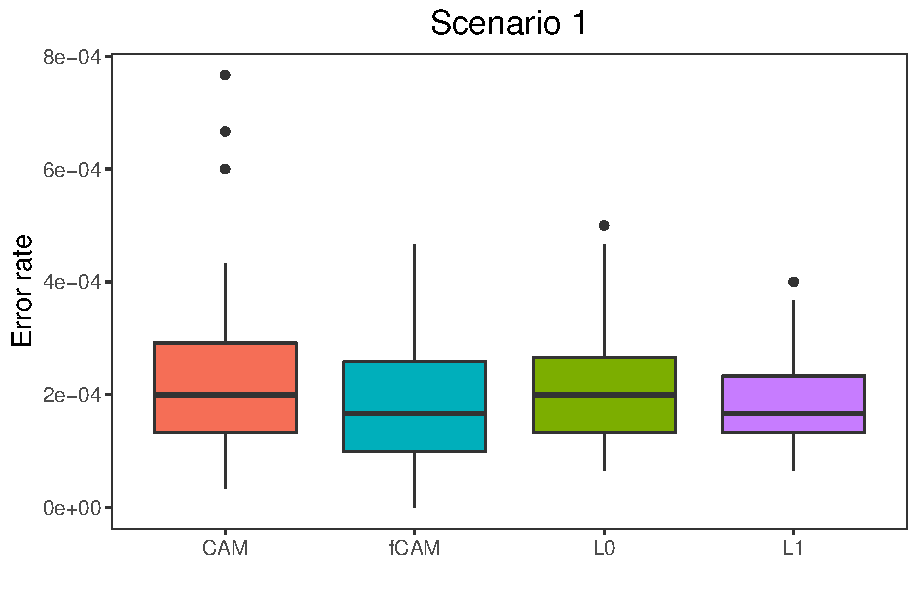
\includegraphics[width = .44\linewidth]{_Images/ch3_err_rate1.pdf}

		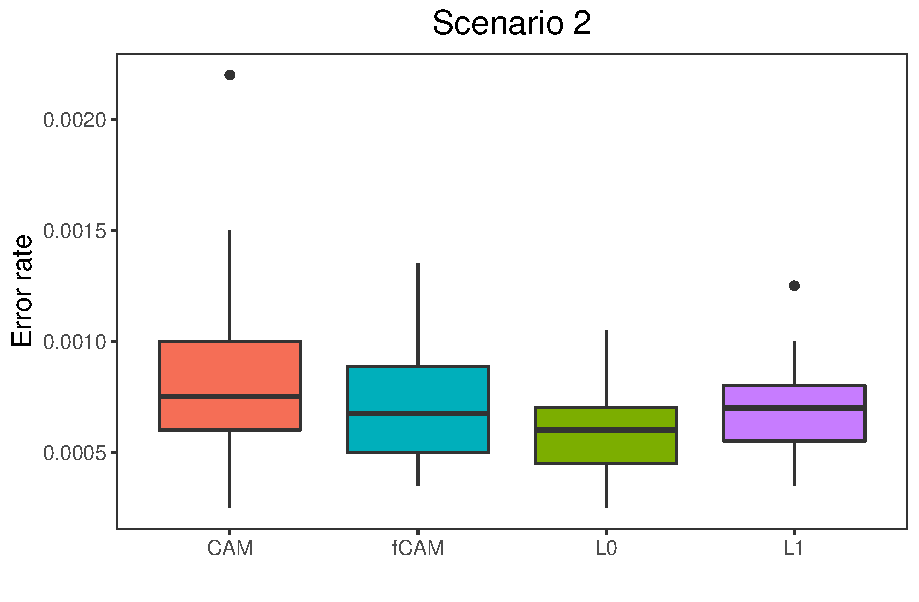
\includegraphics[width = .44\linewidth]{_Images/ch3_err_rate2.pdf}
	}
	\centerline{
		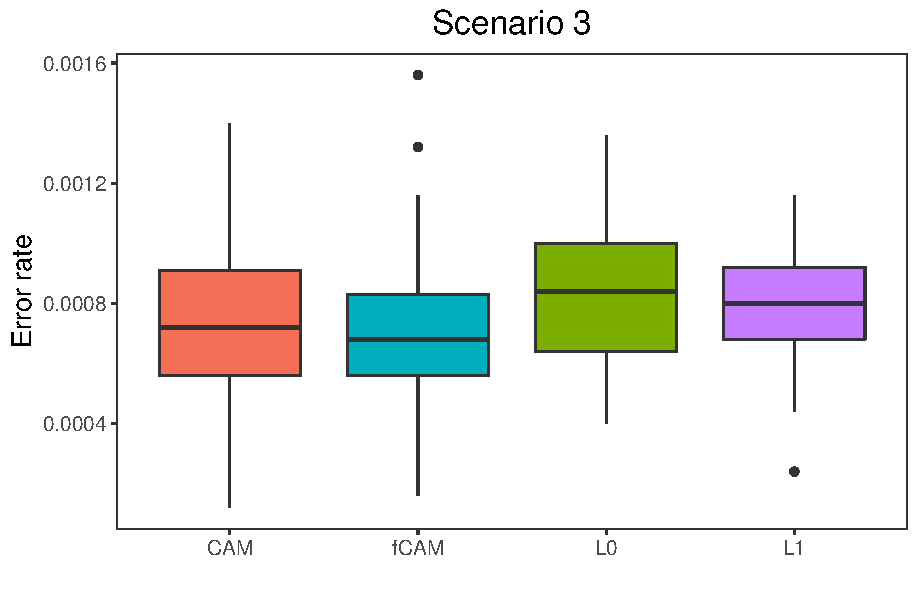
\includegraphics[width = .44\linewidth]{_Images/ch3_err_rate3.pdf}
	}
	\caption[Comparison between the misclassification error rate in the simulation study for the four considered methods.]{Distribution of the misclassification error rate in the simulation study for the four considered methods: CAM, fCAM, and the methods of~\citet{jewell2019} ``L0'' and~\citet{friedrich2017} ``L1''.}
	\label{fig:boxplots_rates}
\end{figure}


To assess the sensitivity of the proposed fCAM to the prior specification, we repeated the numerical experiment for different values of the hyperparameters $h_{A1}$ and $h_{A2}$ in \eqref{eq:G0}. In particular, the shape parameter $h_{A1}$ was supposed to play a key role in the detection of spikes. Keeping fixed the ratio $h_{A1}/h_{A2}$, the parameters were set equal to 3, 4, 6, and 8: a small value implies, \textit{a priori}, less separation between zero and the distribution of the positive spikes while a large value corresponds to the opposite effect. 


Focusing on the classification of each time point as a spike or not, Figure~\ref{fig:boxplots_rates} summarizes the misclassification rate for all competing methods under the three scenarios. The results of the $50$ replications are summarized using boxplots. For our fCAM, we report only the results obtained with $h_{A1} = h_{A2} = 8$ as those obtained for the other choices are essentially equivalent.  The rates are small in absolute value and broadly comparable across the different methods, thus confirming that all the competing models are effective in detecting the spikes.  

However, the proposed fCAM not only enables the detection of spikes but also allows to conduct inference on the clustering structure. Therefore, we report on its ability to identify the clustering structure. Figure~\ref{fig:rand_index} reports the adjusted Rand index~\citep{rand1971,hubert1985} computed on both the observational and the distributional clusters for $h_{A1} = h_{A2} = 8$ (results for other settings are similar). Values of the adjusted Rand index close to 1 denote that the identified structure resemble the true clustering. While for the observational clusters the results are broadly comparable, for the distributional clusters, the performance of the proposed fCAM is uniformly superior. In addition, the variability of the results generally appears to be drastically smaller for the fCAM, thus providing evidence of greater efficiency. This is consistent to the results of \citet{fruhwirthschnatter2020} where  the generalized mixtures of finite mixtures is compared to a standard Dirichlet process mixture model. 

From a computational point of view, the proposed algorithm is clearly more demanding than the optimization methods of~\citet{jewell2019} and~\citet{friedrich2017}.  However, the computing time is comparable to the slice sampler adopted for the CAM, and in general a full run requires just few minutes on a Linux machine with an i7-7700HQ 3.8 GHz Intel processor, 8 GB RAM, running R 4.1.0. For example, for a calcium trace of length 50,000, the computing time of the proposed method is around 2 minutes. Indeed, our experience suggests that the main factor affecting the computing time is the length of the series.  In general, in the analysis of spike activity, we expect the number of clusters  to be small and -- in particular -- much smaller than the number of observations.


\begin{figure}
	\centerline{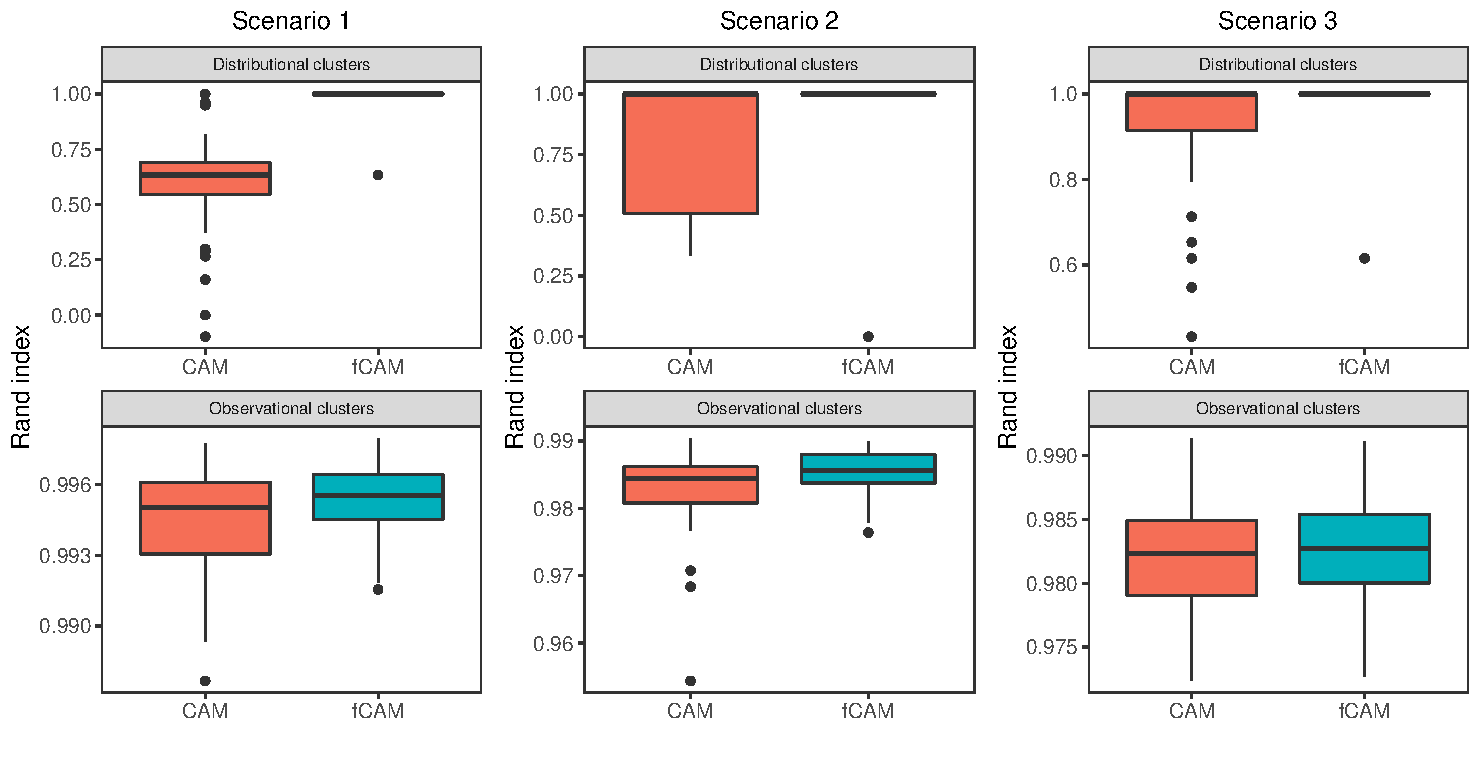
\includegraphics[width = .9\linewidth]{_Images/ch3_rand_index.pdf}}
	\caption[Comparison between the adjusted Rand index of the fCAM and CAM.]{Distribution of the adjusted Rand index on the distributional and observational clusters of CAM and fCAM, computed on the 50 simulations for the three scenarios of the simulated data.}
	\label{fig:rand_index}
\end{figure}



\section{Allen Brain Observatory data analysis}
\label{s:dataanalysis}

\begin{figure}
	\centerline{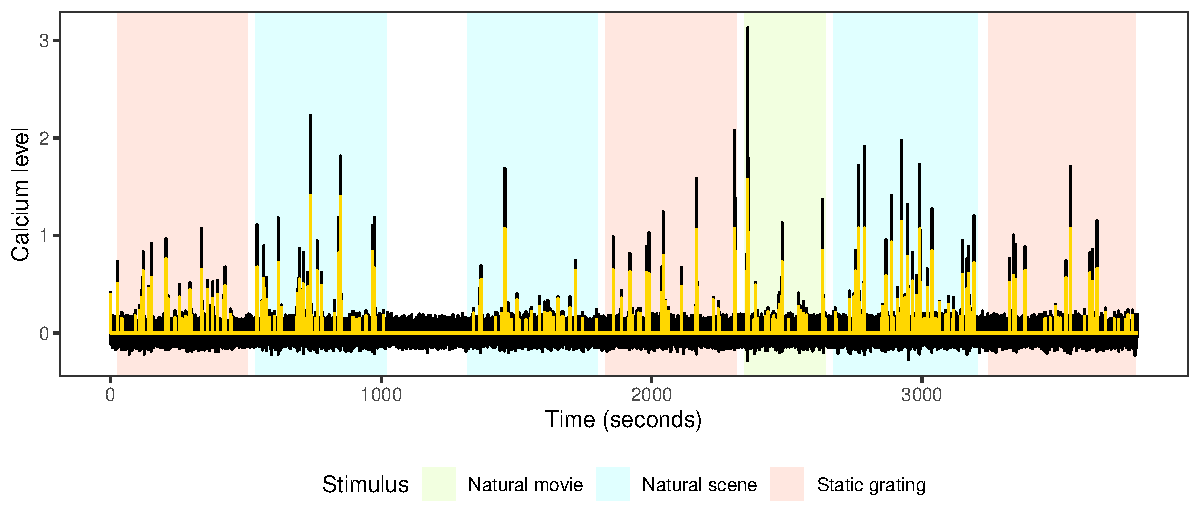
\includegraphics[width = \linewidth]{_Images/ch3_plot_data_new.pdf}}
	\caption[Observed fluorescence trace of a neuron from the Allen Brain Observatory data and estimated neuronal activity.]{Observed fluorescence trace $y_t$ of a neuron from the Allen Brain Observatory data (black line), and visual stimulus to which the mouse is exposed (shaded areas). The yellow line represents the estimated neuronal activity.}
	\label{fig:y}
\end{figure}

We now revert to the analysis of the data from the Allen Brain Observatory~\citep{allen}. The data comprise the $dF/F$-transformed fluorescence trace for a cell during session-B of the experiment. This session comprises three types of visual stimuli (static gratings, natural scene and natural movie) in addition to some period of spontaneous activity (absence of visual stimuli). Since the data are recorded at a frequency of $30$ Hz, the resulting series consists of 113{,}865 time points for a total of 63.2 minutes. 
We focus our analysis on a neuron located in the primary visual area, at an imaging depth equal to 350 microns. %Additional analyses for other neurons are reported in the Supporting Information.
%{\textcolor{red}{ADD SOMETHING LIKE: we focus our analysis for neuron ABC. Additional analyses for other neurons are reported in the Supporting Information. }}

The observed fluorescence trace is shown with a continuous black line in Figure~\ref{fig:y}. Different shaded backgrounds indicate the types of visual stimuli.
Using the notation introduced in the previous Sections, $J=4$ with $j=1, 2, 3$ corresponding to static grating, natural scene, and natural movie, respectively and $j=4$ indicating no stimulus presence. 


We ran the MCMC algorithm of Section \ref{s:posterior_inference} using the same prior specification of Section \ref{s:model} for 15{,}000 iterations discarding the first 7{,}000 iterations as burn-in and keeping one iteration every four to improve mixing.  Visual inspection of the traceplots and Geweke diagnostics showed no issues with convergence. 
%
The superimposed light line in Figure~\ref{fig:y} represents the estimated neuronal activity in terms of the inferred amplitude $A_t$, i.e. removing the measurement errors and the result of the accumulation of calcium from the previous spikes. Here and henceforth, we identified the presence of a spike if the  posterior probability of a spike at time $t$, say $PPS_t$, estimated by the proportion of non-zero $A_t$'s over all MCMC iterations, was greater than  $\kappa=75.5\%$. This threshold allows to control the (estimated) Bayesian false discovery rate at the pre-set value 0.05, that is $\kappa$ solves the equation $$\operatorname{FDR}\left(\kappa\right)=\frac{\sum_{t=1}^{T}\left(1-\mathrm{PPS}_{t}\right) I_{\left(\mathrm{PPS}_{t}>\kappa\right)}}{ \left.\sum_{t=1}^{T} I_{\left(\mathrm{PPS}_{t}>\kappa\right.}\right)}=0.05.$$ For more details, we refer to \citet{newton2004} and \citet{Muller07}. See also \citet{SunReich2015} for a discussion with dependent hypotheses.
%

%
As already mentioned in the Introduction, in calcium imaging it is of interest studying the distribution of the spikes in response to each experimental stimulus, and identifying similarities and differences in these distributions across stimuli. 

We start by investigating the presence of similarities in the neuronal response to different types of visual stimuli. This corresponds to analyzing the clustering of the spike distributions induced by the proposed fCAM. The model clusters together the groups corresponding to the natural scene and natural movie stimuli with high posterior probability, while the static grating stimulus and the absence of stimuli are assigned to two separate distributional clusters. In other terms, the neuron appears to show similar neuronal responses in the natural scene and natural movie stimuli whereas the responses appear distinctly different under the other two conditions. 



To understand whether and how the neuronal response depends on the type of stimulus, we estimated the spike amplitude distribution for each of the four types of stimuli. Figure~\ref{fig:A_distr} shows the histograms of posterior means of the non-zero spike amplitudes for the three types of stimuli. The distribution for the time interval between 1018-1319 sec in Figure \ref{fig:y} (absence of stimuli) is not presented because no activity was detected. Despite the apparent similarities of the distributions in Figure~\ref{fig:A_distr}, the second cluster of spike amplitude distributions (natural scene and natural movie) shows a heavier tail. 
Specifically, the highest observed cluster during the static grating stimulus (top plot) is centered at 1.06, while for the other two stimuli we obtained several higher values, with the largest cluster centered around 1.43. 

%\begin{figure}
%	\centerline{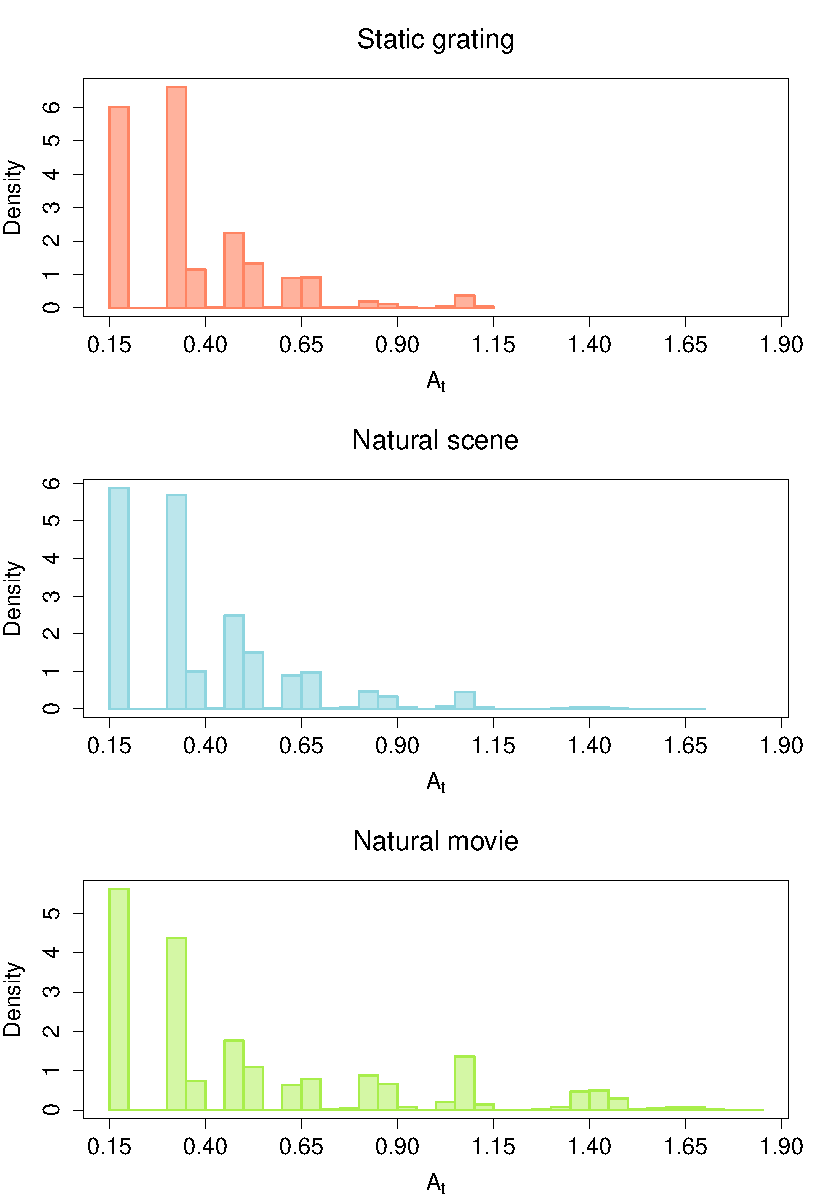
\includegraphics[width = .65\linewidth]{_Images/ch3_hist_new.pdf}}
%	\caption{Empirical distribution of the posterior means of the observational cluster parameters $A_t$ for the three experimental conditions of the Allen Brain Observatory data.}
%	\label{fig:A_distr}
%\end{figure}
\begin{figure}
	\centerline{
		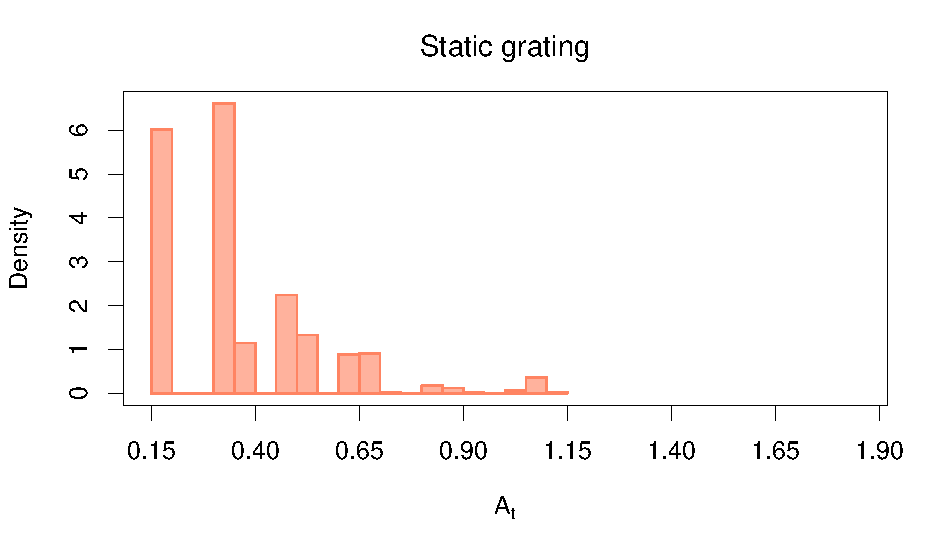
\includegraphics[width = .5\linewidth]{_Images/ch3_hist1.pdf}\hfill
		
		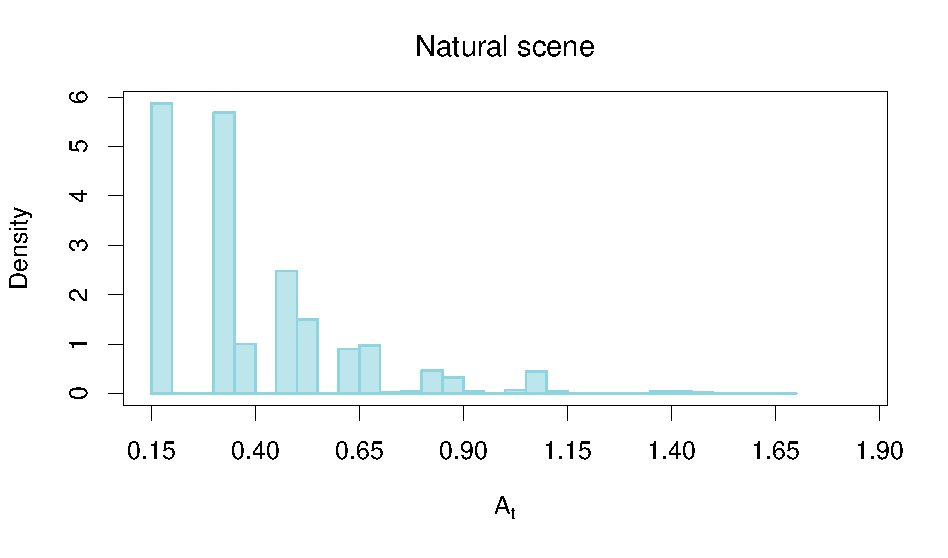
\includegraphics[width = .5\linewidth]{_Images/ch3_hist2.pdf}
	}
	\centerline{
		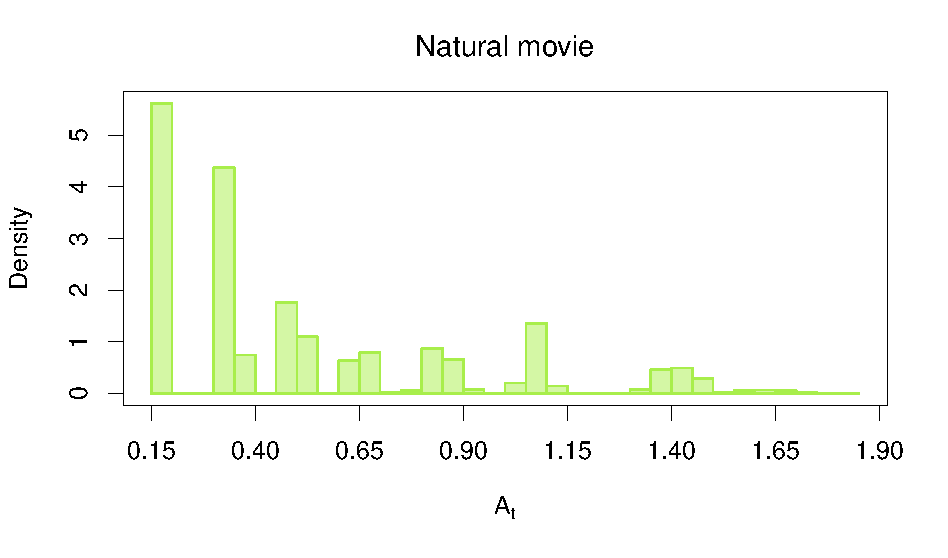
\includegraphics[width = .5\linewidth]{_Images/ch3_hist3.pdf}
	}
	\caption[Distribution of the observational cluster parameters for the three experimental conditions of the Allen Brain Observatory data.]{Empirical distribution of the posterior means of the observational cluster parameters $A_t$ for the three experimental conditions of the Allen Brain Observatory data.}
	\label{fig:A_distr}
\end{figure}

A qualitative representation of how these spike clusters are distributed within the three groups is given in Figure~\ref{fig:spike_color}. The three plots show a short interval of the observed calcium series, chosen in correspondence of one of the highest observed spikes. 
Each plot also shows a series of colored vertical lines: the lines are placed at the estimated spike times, and the colors correspond to the estimated spike amplitudes. 
The represented partition is the posterior point estimate obtained by minimizing the variation of information loss, as proposed in~\citet{wade2018}. Conditionally on the obtained partition, for each cluster a representative value for the cluster parameter is obtained as follows: 
first, for each MCMC iteration, the group-specific average of $A_t$ is computed keeping the partition fixed; then, these values are averaged over all the MCMC iterations.
We notice that for all experiments, high values of the observed calcium level are often produced as the result of several consecutive spikes, since, individually, the spikes are characterized by a relatively low amplitude, and the observed calcium level is cumulated due to its autoregressive behavior.  The autoregressive parameter $\gamma$ has a posterior mean equal to $0.493$ with a 95\% credible interval of $(0.481, 0.505)$.
%
This result corresponds to the understanding that the observed calcium response may be generated by high-frequency firing neurons: due to the low-sampling rate, the non-linear calcium signal essentially captures a super-imposition of multiple spikes \citep{Hoang2020}.  



As a matter of fact, another useful quantity we can compute to compare the neuronal activity between stimuli is the firing rate, which provides a measure of how often the neuron has activated during a specific visual stimulus.
The rate computes the number of detected spikes per second, to take into account the different duration of the experiments.  For the static grating stimulus the posterior mean rate (and related 95\% credible interval) is $0.223$ $(0.216, 0.229)$, while for the natural scene and natural movie stimuli they are $0.419$ $(0.410, 0.428)$ and $0.511$ $(0.495, 0.531)$, respectively. These results highlight the role of spike-frequency adaptation, whereby some neurons show an increased activity when exposed to more complex stimuli, thus exhibiting higher firing rates and larger calcium concentration measurements \citep{Peron2009}.
%



\begin{figure}
	\centerline{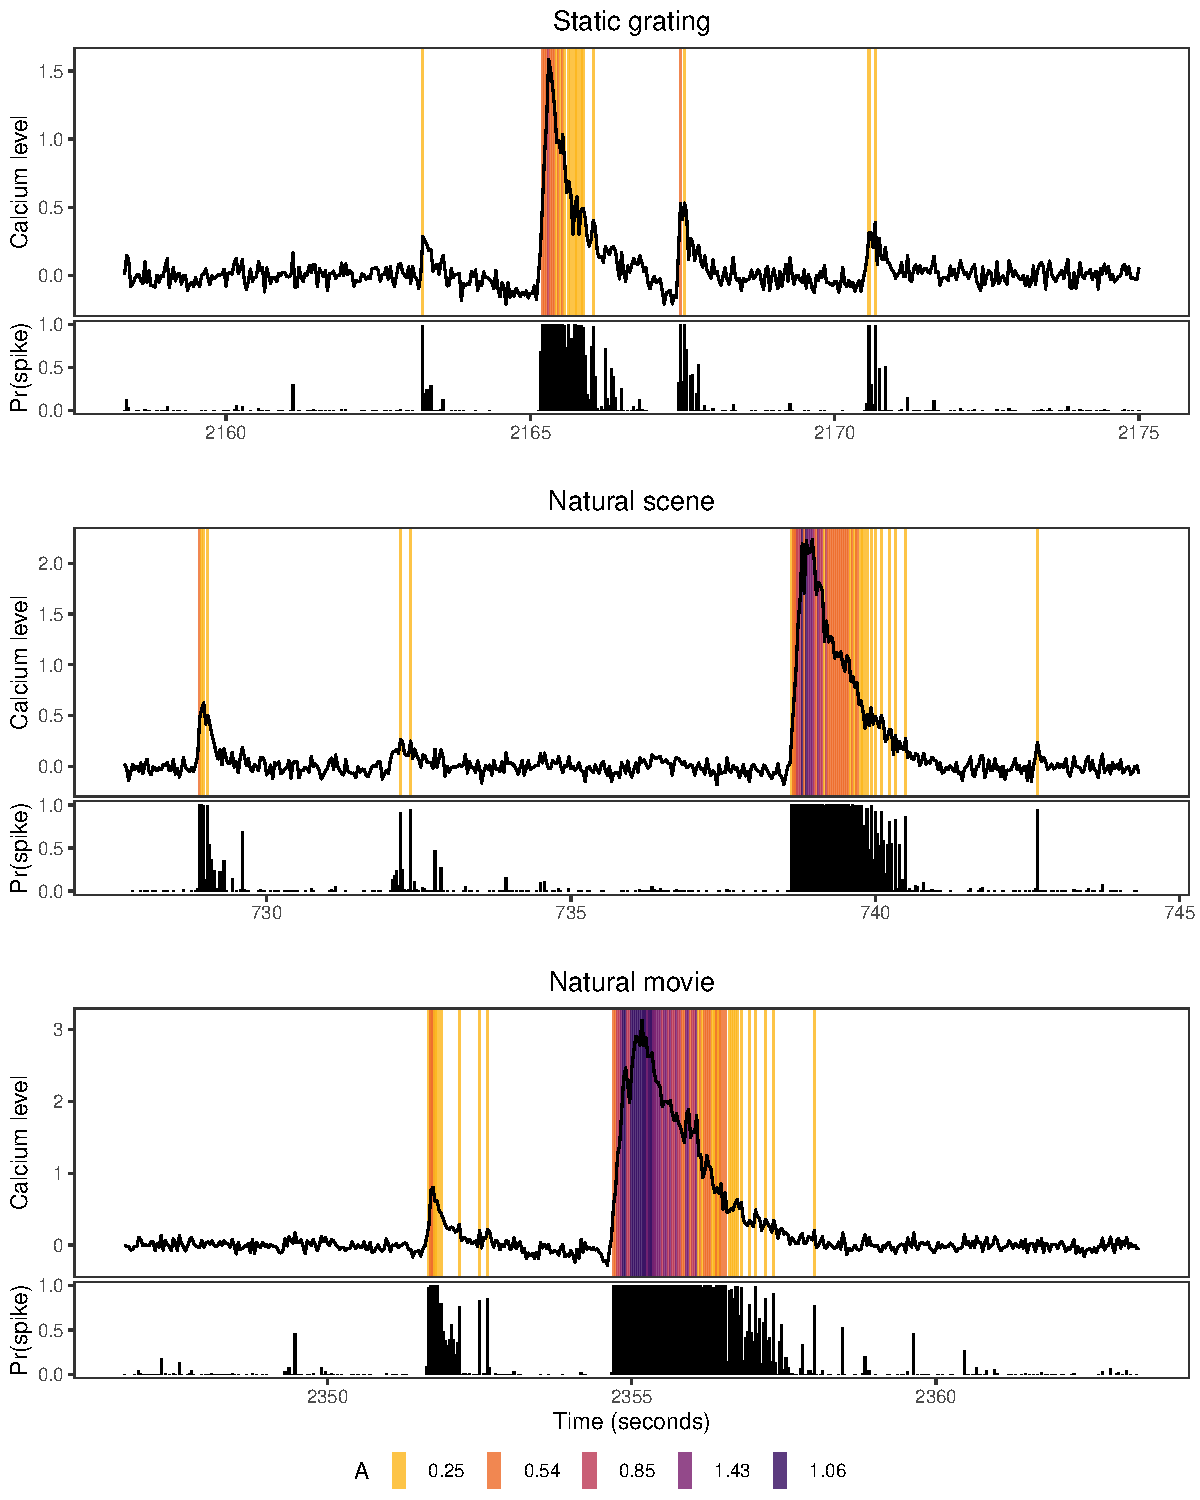
\includegraphics[width = .75\linewidth]{_Images/ch3_spike_color_prob_new.pdf}}
	\caption[Visual representation of the estimated spikes and their amplitudes in the calcium trace from the Allen Brain Observatory data.]{Short interval of length 500 of the Allen Brain Observatory data in correspondence of a spike, for the three stimuli. The vertical lines indicate the time of a spike and the colors correspond to the observational cluster of its amplitude. The bottom panels show the estimated posterior probability of spike presence, for each time point.}
	\label{fig:spike_color}
\end{figure}


















